\documentclass[11pt]{ctexart}


\usepackage[margin=2cm]{geometry}

\usepackage{graphicx}

\usepackage{listings}
\lstset{
	numbers=left,
	numberstyle=\tiny,
	basicstyle=\small,
	keywordstyle=\color{red},
	identifierstyle=,
	commentstyle=color{grey},
	stringstyle=\ttfamily,
	showstringspaces=false
}

\usepackage{url}
\usepackage{hyperref}

\title{\heiti{\LaTeX 总结}}
\author{\kaishu{北方以北}}
% \institute{国家知识产权局专利局专利审查协作河南中心}
\begin{document}

\maketitle

\tableofcontents

\section{序}

这是我关于自己在\LaTeX 学习和使用中笔记的整理和归纳,其中大部分来自于几年间在为知笔记中的收藏记录,少部分来自于其他人的一些课件或文章。这些内容都是零散的,我只是分门别类做了整理,因此如果想系统学习\LaTeX ,最好还是看官方的教程或书籍。

\section{\LaTeX 学习历程}

我从2010年开始接触到\LaTeX ,当时忘记了在哪个地方偶然看到了关于\LaTeX 的一些介绍文章,于是在自己的台式机上下载了\TeX Live,跟着指导一点一点学,但没有学习太深入。2011年上了研究生,我重新拾起了对\LaTeX 的兴趣,开始继续深入的学习,记得当时还去北邮的打印店把整本书都印了出来,并且在数值计算的结课上使用了一个期刊的\LaTeX 模板,老师还高高兴兴地给了我高分。现在想起来,大概是学数学的经常使用\LaTeX ,而其他专业的少人问津,当时的数学老师可能比较惊讶。我记得当时没有使用fontspec和XeCJK库,而是使用了MikTeX包和WinEdt编辑器。到了研究生二年级的时候,我接触了Beamer和XeCJK,并开始应用于幻灯片的制作。但是当时缺少系统和深入的学习,幻灯片制作得并不优雅美观。

我使用\LaTeX 最大的成就,就是用它完成了自己的硕士学位论文。在写学位论文时,我查找了大量的资料,后来使用了北邮一个毕业生的模板,做了稍许的修改。现在看来,\LaTeX 排出来的文章,确实在美观性上远好于Microsoft Word的效果。

工作以后的2014-2015年间,也断断续续地学了一些TikZ,也做了一些幻灯片,同时也全面转向了\CTeX 宏包。但是,由于做文档与单位的风格不同,做幻灯片也不够新颖美观,因此慢慢地少于使用。


我学习\LaTeX 完全出于兴趣,而非学习和工作的需要,并且由于以上断断续续的学习,目前我大概还处于初级使用者的水平,远谈不上深入,而且我预计以后的工作中,也会越来越少地使用\LaTeX ,但作为一项基本的书写技能,现在想把以前零碎的笔记做一个系统化的整理,以方便自己以后的使用,同时也希望有利于其他人的学习。

\section{关于\TeX 作者Knuth的一些轶事}

传说 Knuth 写书写文章的第一稿都是用铅笔写的。 很多人不明白他为什么不用键盘。 其实原因是这样,Knuth 曾经参加过一个训练小秘的学习班,练习打字每分钟 80 个词以上。到了后来,他发现他打字的速度大大高于他思考的速度,所以如果他用键盘,就会出现很多停顿。所以他决定用铅笔,这样可以与读者的思考速度保持一致。 

Knuth 作为一个计算机科学家,为什么放下他所有的工作10年, 专心研究排版美学,创造 \TeX 系统。这是很奇怪的一件事情。其实原因是这样。真正完美的数学排版应该是用金属活字进行的。但是自从70年代以来,真正懂得这项技术的人都死光了。 新的排版机器,很不幸的都被计算机操纵了 (想想 Matrix ) 虽然当时计算机能够排出一些简单的报纸,杂志, 但是它们不能很好的处理数学公式。Knuth 想写出一个小玩艺儿能够在不同的计算机上制造漂亮的数学公式,于是 \TeX (读作 Tech(nology) 的前半部分) 就诞生了。 

很多人都对 \TeX 断行的算法感到满意,其实只有 Knuth 觉得担心。 他设计 \TeX 的时候听说有一本书叫做 Aesthetic Measures,作者是美国 No.1 数学家 George David Birkhoff。 是说怎样用数学公式来衡量“美”。 他查阅了7个Harvard图书馆,其中有一个图书馆有一个拷贝, 但是却被人借走了。无奈,跑到 MIT 去借。还好,借到了。后来他就在 \TeX 里加入了一个变量叫做 badness,用来衡量一行文字的美感。badness 越小这行文字就越美。但是与 Birkhoff 不同,Knuth 对这个公式没有多少信心。也许是因为谦虚。 

Knuth 的书都是自己用 TeX 排版的,但是却不都是自己设计的。传说 Knuth 和 Graham, Patashnik 合作写 Concrete Mathmatics 的时候请了一位有名的图书版面设计家为他们设计好了书的尺寸,字体大小,标题样式, 后来 Hermann Zapf 专门设计了一种数学字体叫做 Euler, 自此,数学家 Euler 的灵魂浮游于 CM 当中…… 另外一个图书设计家告诉 Knuth 一种格式数学公式的办法, 就是不把数学居中,而是只相对正文缩进一定距离。 


大家都知道 1974 年图灵奖授予 Knuth 主要是因为他写了一部巨著叫做 The Art of Computer Programming 但是不幸的是,很多人不能理解,甚至不相信他为这部书起了这么一个不“科学”的名字。 后来很多人的著作里出现这样的文献引用:"The Act of Computer Programming, Donald Knuth." 

Knuth 是个喜欢自夸的人,这是毫无疑问的。 在他出版 The Art of Computer Programming 之前就已经有这种苗头了。 还没有出版的时候,在一次会议上,有个人知道他的这种性格,就说:“我猜你正在写的这本书的书名肯定是 ‘An Introduction to Don Knuth’。” Knuth 回答说:“正好相反。我要以你的名字来命名它。” 原来这个人的名字叫 "Art Evans". 

Knuth 是Caltech数学系博士毕业的 但是他常常说:“我戴着一顶计算机科学家的帽子,而不是一顶数学家的帽子。” 这说明他似乎对数学家有某些看法。在他看来数学家只知道“What is it”,而他还知道 "How to do it". 这就是他认为的数学与计算机科学的区别。

Knuth 回到 Stanford 时,学校让他自己给自己一个头衔,他就选了一个 Professor Emeritus of The Art of Computer Programming 他其实觉得“计算机科学”不是科学。 虽然大家很希望计算机编程变成科学,这是某ACM刊物提出的忠旨。但是 Knuth 觉得奇怪为什么大家这么喜欢科学,以致于他们瞬间把程序设计变成了科学,方法就是叫它“计算机科学”。Just call it "Computer Science" 在他眼里,计算机科学其实仍然是门艺术。 在 Knuth 的眼里,科学与艺术有什么区别呢? 艺术是人创造的,而科学不是。 艺术永远是可以无止境的提高的,而科学不是。 艺术需要天赋才能掌握,而科学不需要,按部就班就行。所以,The ... ART ... of Computer Programming! 



Knuth 的 The Art of Computer Programming(TAOCP),开始写的也不那么好。 传说有一天 Bob Floyd 给 Knuth 一封信,开门见山就说: “Don, 请不要用那么多感叹号!”信的结尾至少打了五个概叹号。 看了之后,Knuth 发现 TAOCP 里竟然平均每页有两个感叹号!! 

有人说 Knuth 写完三卷 taocp 就去研究 TeX,其实是因为害怕写第四卷。很多人早就希望他放下 TeX,继续写书。 Knuth 说:“一个人要把事情做的完美,只有当他跟上帝的意图保持和谐,现在上帝要我去写第四卷了。” 

Knuth 很推崇随机算法。他批改作业时,一般都是翻到随机一页,仔细看那一页, 之后就对学生的作业有了一个概貌,其它的部分就看的不那么仔细了。Knuth 看书的时候首先看第316页,如果书很短就看第100页。仔细看那一页。之后他就可以说那本书好不好。 据说这样做出判断的正确率很高。不知道是否有很多人跟他学,看316和100. 以后写书要注意把第316页或者100页写好呀! 

你们知道 Knuth 发明了一种程序设计方法叫做 Literate Programming (文学编程) ,把程序当成文学作品来写。这样可以创造永恒的作品, 甚至几十年后还有人用它作为茶余饭后的读物。 他为什么要发明这个东西。原因有2: 1. 他想让一个程序员(也许是他自己)在某一天拿到普利策奖。 2. 他想让提出“Structured Programming”(结构化程序)的那些家伙 在写“非文学程序”的时候,就像他当年写“非结构化程序” 的时候一样觉得自己有罪。 



他的“文学编程”思想最早是在英国 Computer Journal 发表的。 当人问他为什么不在美国发表。他说,美国人没文化,他们不能理解这个东西。 






Knuth 喜欢在他的作品里用 "we" 作为主语, 虽然很多时候文章是他一个人写的。 有人认为使用被动语态好。但是 Knuth 认为不应该大量使用被动语态。 “用 We 可以减少被动语态带来的麻烦。‘we’是指你和你的读者。” 那么怎么称呼作者?答案是: the authors, the first author, 或者直接用名字。 但是他确实反对使用 "I",除非你是身名显赫, 人人尊敬的君王式人物,否则最好不要在论文里用 "I"。 在你描述你的程序时,喜欢说 "we insert the element in the heap" 还是 "it inserts the element in the heap" ? Knuth 总是喜欢用 "we"。显然他已经融于算法的动作之中了。 

虽然他不喜欢论文里用 "I", 但是他喜欢让他的程序自称 "I". 看这里: 


\begin{verbatim}
This is TeX, Version 3.14159 (Web2C 7.3.7x) 

! I can't find file `kkkk.tex'. 

<*> kkkk.tex 



Please type another input file name: 

\end{verbatim}





有很多人跟着他学,把这种称呼顽皮的发挥到极致: 
\begin{verbatim}
Welcome to Scheme 48 0.57 (made by wy on 日 11月 24 13:20:27 CST 2002). 

Copyright (c) 1993-2001 by Richard Kelsey and Jonathan Rees. 

Please report bugs to [email]scheme-48-bugs@martigny.ai.mit.edu[/email]. 

Type ,? (comma question-mark) for help. 

> (define (sq x) (* x 

x)) 



; no values returned 

> 

Exit Scheme 48 (y/n)? <按 Ctrl-D> 

I'll only ask another 100 times. 

Exit Scheme 48 (y/n)? 

I'll only ask another 99 times. 

Exit Scheme 48 (y/n)? 

I'll only ask another 98 times. 

Exit Scheme 48 (y/n)? 

I'll only ask another 97 times. 

Exit Scheme 48 (y/n)? 

I'll only ask another 96 times. 

Exit Scheme 48 (y/n)? 

I'll only ask another 95 times. 

Exit Scheme 48 (y/n)? 

I'll only ask another 94 times. 

Exit Scheme 48 (y/n)? 

...... 

\end{verbatim}



Knuth 有一次布置了一个作业,要求在两个星期以内做出一个用于控制时代广场那种 8x256 像素的阵列显示屏幕的系统, 并且写出一个用户手册。这个用户手册必须让不懂电脑的人也能看懂。 作业交上来以后 Knuth 把文档拿给他夫人(Jill Knuth)看, 结果发现 Jill 对文档里的 "Menu" 和 "Scrolling" 这样的单词都摸不着头脑, 更不要说 "left-indented", "exit", ... 



Knuth 曾经在 American Mathematical Monthly 发表过一篇叫做 "The Toilet Paper Problem" 的论文, 据说是一个研究怎样合理使用厕纸的算法。 现在收录于 Selected Papers on Analysis of Algorithms, p.111 。这篇论文投到 Monthly 时,在节标题使用了大量“粪便学”词汇。 编辑警告 Knuth 说,笑话在我们这里是危险的,请你三思! 不得已啊,Knuth 后来把小节标题里的那种词改掉了。 可是他很不想改文章的标题。 怎么办呢? 他给编辑一封信说,我已经以这个标题做过两次演讲, 这个主题已经被广泛的采用和讨论……云云。 最后编辑回信说:“你的厕纸被接受了!” 


Stanford 计算机科学系楼里的厕纸架上可以并排放两筒厕纸。 人上厕所时有可能从两个中的一个取纸。 两个卷筒不一样大的时候,喜欢从大的那筒拿纸的人叫做 big-chooser 喜欢从小的那筒拿纸的人叫做 little-chooser。 如果两筒大小差不多,一般人都会从离自己最近的那筒取纸。 厕纸用完的时候一般由janitor(门口老大爷?)提供新的纸。 如果一边的用完了,那就换掉那一边,如果两边同时用完,那么有人就有麻烦了……Knuth 似乎在计算那种两筒同时用完的窘境出现的概率…… 论文原文的一个拷贝在: \url{http://learn.tsinghua.edu.cn/homepage/015450/doc/toiletPaperProblem.pdf}比较复杂的数学…… 有兴趣的可以看看。 另外,Don Norman 在这里有一些新设计的厕纸筒可以避免这种情况发生: \url{http://www.jnd.org/dn.mss/ToiletPaperAlgorithms.html}看来 Knuth 是在白费工夫。应该授予 IgNobel 或者 IgFields 


Knuth 和 Graham 他们合写的 Concrete Mathematics 本来不会做的那么花哨的。结果后来他们专门为那本书设计了字体,页面样式, 所有习题都给出了出处。几乎所有页面都至少有一个涂鸦, 连《爱利丝漫游奇境记》都被列入参考文献…… 这是怎么回事呢?原因就是 Knuth 在写书期间去看了一部电影: “白雪公主与七个小矮人”。 看完之后 Knuth 感叹道: 难以置信,这样完美的艺术品竟然可以在1937年完成。 我一定要把我的书做成一个艺术品,而且要在三个月之内完成!结果他说到做到了。

\section{\LaTeX 基本语法拾遗}
\LaTeX 是向后兼容的。

\subsection{引用宏包}
nag宏包。事实上,如果你的代码没问题,这个宏包将不会做任何事情。注意:把这个宏包放在你的导言区的第一行(甚至在 \verb|\documentclass| 之前)。它将会检测你文档中是否使用已经被淘汰了的宏包以及过时的命令。

\subsection{排版基础}


在paper开头,必不可少的是会引用LaTeX packages。除了常用的\LaTeX 包,在此需要特别说明的有两个:一是\verb|\usepackage[american]{babel}|,另一个是\verb|\usepackage{microtype}|,引用这两个包会大大提升排版的正式程度和美观程度。其中\verb|\usepackage[american]{babel}|的引用是遇单词换行的时候,确保单词的切割是按照音节来而不是随意切割。这会让作为native speaker的审稿人赏心悦目,心中暗爽。而\verb|\usepackage{microtype}|的最大特点就是能够调整全篇文章(或局部)的字间距,字间距最大调整范围为±1em。可使得某段落不会出现单独一个单词占一行,或文章末尾单独一行文字占一页的不美观情况。\footnote{该包在NIPS中自带引用,而ECCV由于LNCS在排版方面的一些限制因素,不推荐在ECCV中使用该包引用}如果有使用到字体宏包,需要将 microtype 宏包放在它们的后面,因为这个宏包对单词、字母的调整和字体是有关的。

在行文过程中若使用括号,括号前一定要有空格与前文内容分开。这也是中文作者很容易忽略的一点。例如,“the boosting algorithm (AdaBoost)” “the clustering algorithm (k-means)”。

siunitx 宏包大大简化了写作科技文的 \TeX 命令,科技文写作中很大一部分是单位、数字。这个宏包添加了一些命令,比如 \verb|\num|命令可以输出我们想要的各种方式的数字形式(比如科学记数法),而 \verb|\si| 命令用来输出单位。我经常用到的命令是 \verb|\SI| 和 \verb|\SIrange|。比如 \verb|\SI{10}{\hertz}| 输出为 “10Hz”(这能有效避免输入错误,我可能会写成 HZ 或者 hz 而不是 Hz)。\verb|\SIrange| 命令多一个参数:\verb|\SIrange{10}{100}{\hertz}| 输出为 “10Hz to 100Hz”。

hyperref 非常强大,你可以有非常多的可能性,其中最突出的特色是超链接。当引用一幅图的时候,引用与图形形成了链接,当你点击引用的地方,它会跳转到链接的图片处。并且 hyperref 可以让你插入 PDF 元数据到你的最终文档中。注意:作为一个经验法则,你应该在导言区的最后加入这个宏包,在所有宏包之后。也存在少数例外的情况:比如,cleveref宏包应该在 hyperref 之后。

单双引号的使用。正确的单引号使用方式:左引号为 (全键盘上数字1左侧键位),右引号为 ' (分号右侧键位)。双引号则重复输入两次即可(即 '')。切记不是平常引号的输入方式。

脚注使用时如遇句尾,则应该在句尾标点符号后引用,具体为:“respectively.\verb|\footnote{blablabla}”|。这样是为了防止句尾是数字的情形产生误读:如果是数字,footnote的标号就很可能被误认为数字的次方。

一些英文简写的用法。“that is”写作“i.e.,”,“for example”写为“e.g.,”,而“参看/参考”简写为“cf.”。注意,前两者有两个“.”且末尾要有“,”而“参考”的简写只有一个“.”。

文中在引用参考文献时要用“\~{}”(而不是直接空格)来产生空格。例如,“state-of-the-art MIL algorithms, e.g., miFV\~{}\verb|\cite{bibmiFV}| and miGraph\~{}\verb|\cite{bibmiGraph}|, and …” 用“\~{}”来产生空格的好处是使得“miFV [5]”作为一个整体,在换行时不会发生“[5]”与前文分开而单独处于行首的错误情况。“\~{}\verb|\ref{}|”命令同理。

注册商标外面那个R带一个圈可以写为\verb|\textregistered|(注册)或\verb|\texttrademark|(商标),也可以使用\verb|\textcircled{\scriptsize R}|。

为产生目录中的简写形式,可使用\verb|\caption[short text]{long text}|,其中方括号中为简写形式。

段落结尾时,不要使用\verb|\\|,使用双反斜杠是为了本段继续书写。

如果编译时出错,可在出错前的命令前添加\verb|\protect|用于调试,但应修复错误。

\LaTeX 类及宏包是在\verb|\leftmark|和\verb|\rightmark|中存储章节编号的。

为改变输出尺寸,可使用\verb|landscape|宏包。页面布局可使用宏包\verb|typearea|。页面间距可使用\verb|geometry|宏包。



英文中常用到连笔,但有些PDF阅读软件并不支持连笔的搜索和复制,此时可在\verb|microtype|宏包中设置\verb|noligatures|选项来进行取消。

命令\verb|\xspace|可根据不同的情形添加空格:后面跟一个单词时,加入一个空格;如果后面是英文的句号、逗号、叹号和引号则不添加空格。



\subsection{行间距与段间距}

LaTeX  支持的长度单位有:
\begin{itemize}
	\item in - 英寸(inch)(
	\item mm - 毫米(millimeters)
	\item cm - 厘米(centimeters)
	\item pt - points (大约 $1/72$ inch)
	\item em - 接近当前字体的字符 "M"的宽度(approximately the width of an "M" in the current font)
	\item ex - 接近当前字体的字符 "x"的高度approximately the height of an "x" in the current font
\end{itemize}
长度也可以是负值, 例如  -1.5em.  注意到数字 0 本身不是一个长度,  必须表明是0in 或 0pt 等.

\LaTeX 默认行间距为行高的20\% ,为调整行间距,可使用\verb|setspace|宏包,其具有选项\verb|onehalfspacing|可将行间距调整为1.5倍行高。宏包\verb|parskip|可用于取消\emph{段落}的缩进,此宏包中还包括段落间的距离调整功能。

段落间距有关变量:
\begin{itemize}
	\item \verb|\baselineskip|:行基线间距。
	\item \verb|\lineskip|  :行间距。
	\item \verb|\baselinestretch|:伸展因子。
	\item \verb|\parskip|:部分段间距。
	\item \verb|\lineskiplimit|:当两行字之间的距离小于\verb|\lineskiplimit|时,行距自动设为\verb|\lineskip|。
\end{itemize}
其中段间距等于\verb|\lineskip| + \verb|\parskip|,行间距等于\verb|\lineskip| = \verb|\baselineskip| 乘以 \verb|\baselinestretch|

一般在中文文章中,将 \verb|\parskip| 设置为 0pt,即行间距和段间距相等。设置伸展因子调整行距比较不靠谱,因为经常调不对,索性直接通过 \verb|\fontsize| 直接调 \verb|\baselineskip|,使得 \verb|\baselinestretch| 一直是1,倒来的精确。通过设置伸展因子调整行距不靠谱的原因是默认的 \verb|\baselineskip| 大于字体大小,因此如果你伸展因子设置为 1.5,则实际得出的行距要大于 1.5 倍行距,示例如下:
\begin{lstlisting}
\renewcommand{\baselinestretch}{xx}:设置伸展因子。
\renewcommand{\baselinestretch}{1.5} \normalsize:不改变字体大小,只改变行距。
\end{lstlisting}

通过在源文件中输入 \verb|\showthe\baselineskip|,可以在编译时得到当前的\verb|\baselineskip|的值,并显示出来(在编译时会停住,显示 \verb|\baselineskip| 的值)

\subsection{对齐}
一行对齐:\verb|\leftline{左对齐}| \verb|\centerline{居中}| \verb|\rightline{右对齐}|

多行或者段落对齐:
\begin{itemize}
	\item 左对齐 \verb|\begin{flushleft}...\end{flushleft}|
	\item 居中 \verb|\begin{center}...\end{center}|
	\item 右对齐 \verb|\begin{flushright}...\end{flushright}|
\end{itemize}

\subsection{页眉页脚}
普通的页眉页脚可以使用\verb|\pagestyle{plain}|或\verb|\pagestyle{headings}|,前者不产生页眉页脚,后者产生普通的页眉页脚。

为产生更丰富形式的页眉页脚,可使用fancyhdr宏包来定制,引入宏包后使用\verb|\pagestyle{fancy}|来定制具体的格式。

使用中发现footnote会被分页,可以在某处添加\verb|\interfootnotelinepenalty=10000|来禁止。

\subsection{字体}
使用命令\verb|\sffamily|可将当前字符的字体切换为无衬线字体。

早就有人写了完整的LaTeX字体巡礼:\url{http://www.tug.dk/FontCatalogue/ },这个网站罗列了156个LaTeX中可以免费使用的字体,并且给出了例子和调用的源代码,需要注意的是这些字体并非默认安装在机器上,但至少都能从CTAN得到——不光是宏包,还有字体文件(因为像winfonts,MinionPro这些宏包需要用户自己拥有相应的字体,CTAN上并没有)。 

推荐一下几个字体/字体包:
\begin{description}
	\item[Palatino] Will Robertson的文档总是用Palatino,这字体的名气也不小。胖胖的很活泼,笔锋也优雅,有羽毛笔的进化痕迹。LaTeX中最省事的是用 \verb|\usepackage{mathpazo}| 来统一修改正文和数学字体,这个宏包还有 \verb|[sc, osf]| 参数,分别对应小大写字母和不齐线数字。此外还有一个palatinox宏包可以直接调用Windows系统中的Palatino Linotype(这是微软认证发布赫尔曼·察普夫的原作),相关网址是:\url{http://www.ctan.org/tex-archive/fonts/truetypemetrics/palatinox/},需要手动安装。在这个URL的上一层还能看到另一个经典字体frutiger,只是我手头没有Linotype Frutiger。 
	\item[Garamond] 1530年诞生的经典字体,LaTeX中通过mathdesign可以使用: \verb|\usepackage[garamond]{mathdesign}| 来使用。Garamond字体十分大气,打印在纸张上也特别好看,法国很多口袋图书用的是Garamond。 需要注意的是虽说免费,URW的garamond字体在默认安装的发行版中可能不存在,但是可以下载到,例如\url{http://ctan.binkerton.com/nonfree/fonts/urw/garamond/ }下载所有pfb文件:ugmr8a.pfb ugmri8a.pfb ugmm8a.pfb ugmmi8a.pfb 放到 \verb|font\type1\| 里面的某个目录后刷新数据库即可 
	\item[Times] 除了 \verb|\usepackage{times}| 外,\verb|\usepackage{mathptmx}| 可以把数学字体也改成类似Times的字体。这个字体真的不需要再多说什么了,总之我觉得看久了眼睛会累,但是打印的效果非常稳妥。
	\item[Utopia] Utopia有点像Times,但更宽敞一些。\verb|\usepackage{fourier}| 统一修改正文和数学字体为Utopia, \verb|\usepackage[adobe-utopia]{mathdesign}| 则是mathdesign的调用方法,差别不太明显。
	\item[Avant Garde/Courier/Bookman/New Century Schoolbook] 
不是我懒,这几个字体在PSNFSS中是可以搭配着用的:\verb|\usepackage{avant}| 只载入Avant Garde,\verb|\usepackage{bookman}| 则同时载入Bookman(衬线),Avant Garde(无衬线)和Courier(等宽)字体,\verb|\usepackage{newcent}| 同时载入New Century Schoolbook(衬线),Avant Garde(无衬线)和Courier(等宽)字体 
	\item[Charter] 十分饱满的衬线字体,适合屏幕阅读。\verb|\usepackage{charter}|
	\item[Helvetica/Optima] 这两个字体放一块是因为我觉得它们是无衬线字体,比较适合用来作幻灯片。Helvetica可以 \verb|\usepackage{helvet}| , Optima没有写成宏包的形式,就可以用 \verb|\renewcommand{\sfdefault}{uop}| ,然后 \verb|\renewcommand*\familydefault{\sfdefault}| 来调用。在幻灯片这样的尺寸上,Optima变化的线宽才显现出优美来。 (不过beamer的作者认为Optima不适合做幻灯片)
	\item[其他] 建议看看\url{ftp://tug.ctan.org/pub/tex-archi … t_Survey/survey.pdf} 这篇文章,介绍得相当详细,而且有效果图展示。 
	\item[Minion Pro] \url{http://tug.ctan.org/tex-archive/fonts/minionpro/} 有详细的安装说明,只要不出错是肯定能安上的,装了Acrobat Reader 7.0以上的用户都能在Acrobat安装目录下找到 MinionPro-Bold.otf , MinionPro-BoldIT.otf , MinionPro-It.otf , MinionPro-Regular.otf 这四个文件,按照安装说明拆解它们四个已经能满足日常文档的需要。此外,MnSymbol宏包(MiKTeX可以自动安装)是配合Minion Pro的数学宏包,最好装上,不过 \verb|\usepackage{MinionPro}| 就够了,会自动载入MnSymbol宏包。
\end{description}

其实用来用去才发现,LaTeX自带的这些字体才是真正经过时间和实践检验的经典字体,是TUG智慧的结晶。而且,这150多种字体也涵盖了绝大部分(LaTeX能触及到的)字体使用领域。这是不应该被遗忘的宝藏。

\subsection{数学公式排版}
文中,特别是在equation环境下,如果要插入公式,则公式后一定要有标点“逗号”或“句号”。使用方法:在公式后加入“\verb|\,,|”(逗号)或“\verb|\,.|”(句号)即可。不推荐使用\verb|\text{,}|或\verb|\text{.}|。因为\verb|\text{}|环境下的标点长相与“\verb|\,,|”或“\verb|\,.|”不同,且“\verb|\,,|”或“\verb|\,.|”前会自动与公式隔出一段距离,更加正式、美观。

公式中的\verb|\ldots|和\verb|\cdots|。“\verb|\ldots|”是列举中的省略符号,而“\verb|\cdots|”用于运算(如连加、连乘等)中的省略,二者主要区别在于位置一高一低,切勿混用。

公式中如果有指数或对数表示,要用\verb|\exp|或\verb|\log|命令。不能用\verb|\text{exp}|或\verb|\text{log}|,更不能直接输入exp或log来表示。

在很多机器学习和视觉文章中会用到范数,正确的一范数或二范数表示应为\verb|$\ell_1$或$\ell_2$|,输出为$\ell_1$或$\ell_2$。

公式中的单位向量或零向量要用向量写法:\verb|\vec{1}| 或\verb|\vec{0}|,有时也用\verb|\bm{1}|加粗来表示向量,否则会被误认为标量。

\verb|\left \right|:可以用.匹配不存在的左右部分 

矩阵分块:在array环境中加线,类似tabular, 

虚线:用arydshln宏包 

用\verb|;{}|代替竖线条 

用\verb|\hdashline|代替代替\verb|\hline|,或下载pmat宏包

图\ref{fig:greeks}是希腊字母的命令表示。
\begin{figure}[htpb]
\centering
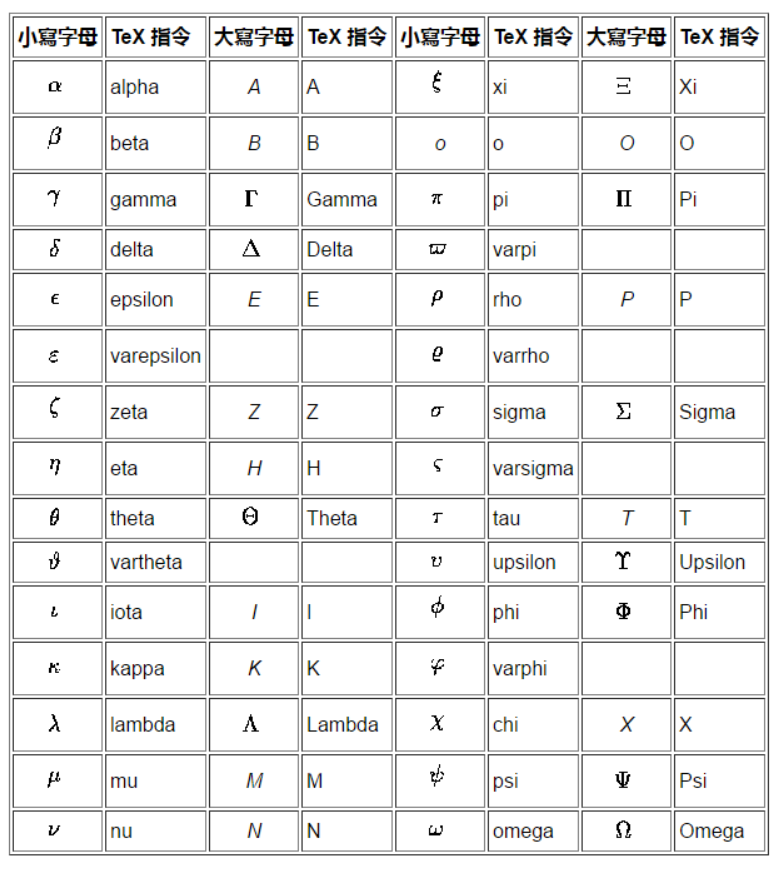
\includegraphics[width=0.7\linewidth]{greeks.png}
\caption{希腊字母的命令表示。}\label{fig:greeks}
\end{figure}

\subsection{列表环境}
类型有三种:itemize,enumerate和description。

默认的列表环境空白较大,如果需要更紧凑的列表方式,可以选用 mdwlist 宏包提供的 \verb|itemize*|、\verb|enumerate*| 和 \verb|description*| 环境,用法和无星号的版本一致。

在列表的内部,很容易改变一些距离
\begin{lstlisting}
\begin{itemize}
 \setlength{\itemsep}{1pt}
 \setlength{\parskip}{0pt}
 \setlength{\parsep}{0pt}
 \item first item
 \item second item
\end{itemize}
\end{lstlisting}

枚举的列表计数可以通过其计数器来改变。enumerate 提供了四个计数器 enumi,enumii,enumiii, enumiv 对应不同层次的枚举。下面的示例会产生第5个计数:
\begin{lstlisting}
\begin{enumerate}
 \setcounter{enumi}{4}
 \item fifth element
\end{enumerate}
\end{lstlisting}

\subsection{表格排版}
表格的多列示例:
\begin{verbatim}
\multirow{number of rows}{width}{entry text}
\multicolumn{number of columns}{formatting options}{entry text}
\end{verbatim}

如果想让标题放在表格的上方就把caption加在\verb|\begin{table}|和\verb|\begin{tabular}|之间,如果想把标题放在表格下方,就把caption放在\verb|\end{table}|和\verb|\end{tabular}|之间。

想在表格下方加以段话的话,就在\verb|\end{tabular}|和\verb|\end{table}|直接加一句话,有时候要用\verb|\newline|,有时候不用。但加的这段注释有时候是doublespace的,想变singlespace,加一句\verb|\linespread{1}|就行了。

\subsubsection{彩色表格}
使用\verb|colortbl|宏包可制作彩色表格,主要使用的命令是\verb|\columncolor|和\verb|rowcolor|,前者给列进行着色,后者给行进行着色。代码如下\footnote{参见\url{http://tex.stackexchange.com/questions/176220/fancy-colored-array-in-latex}}:
\begin{lstlisting}[language=tex]
\documentclass[a4paper,12pt]{article}
\usepackage[left=1.5cm,right=1.5cm,top=1.5cm,bottom=1.5cm,ignoreheadfoot]{geometry}
\usepackage{array}
\usepackage[svgnames,table]{xcolor}
 
\newcommand*{\arraycolor}[1]{\protect\leavevmode\color{#1}}
\newcolumntype{A}{>{\columncolor{blue!50!white}}c}
\newcolumntype{B}{>{\columncolor{LightGoldenrod}}c}
\newcolumntype{C}{>{\columncolor{FireBrick!50}}c}
\newcolumntype{D}{>{\columncolor{Gray!42}}c}
 
\begin{document}    
 
\begin{center}
\sffamily
\arrayrulecolor{white}
\arrayrulewidth=1pt
\renewcommand{\arraystretch}{1.5}
\rowcolors[\hline]{3}{.!50!White}{}
\begin{tabular}{A|B|C}
  \multicolumn{3}{D}{\bfseries Example table}\\
  \rowcolor{.!50!Black}
  \arraycolor{White}\bfseries First column &
  \arraycolor{White}\bfseries Second column&
  \arraycolor{White}\bfseries Third column\\
  1 & A & E\\
  2 & B & F\\
  3 & C & G\\
  4 & D & H\\
\end{tabular}
\end{center}
 
\end{document}
\end{lstlisting}

得到的表格图\ref{fig:colortbl}所示。
\begin{figure}[htpb]
\centering
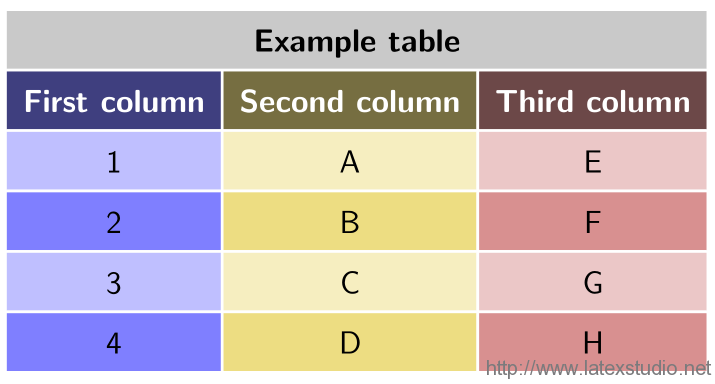
\includegraphics[width=0.5\linewidth]{colortbl.png}
\caption{彩色表格示例。}\label{fig:colortbl}
\end{figure}


\subsection{插图排版}
若文章需要插入很多图片,那么直接和\verb|“.tex”|放在一起就会很杂乱。这时可在\verb|”.tex”|所在目录下新建名为“figure”的文件夹,将图片放入figure文件夹后调用\verb|\graphicspath{{figure/}}|命令即可。

可将\verb|\vspace{-1em}|放置于figure或table的\verb|\caption|和图片或表格主体之间,来缩小空白节省篇幅。当然,如果会议或期刊明确要求了图片主体与图片标题的间距,则不要使用该命令!

插入图片时需要估算本页还有多少空间可用,下面的示例可以根据这个空间来确定图片的高度:
\begin{verbatim}
\includegraphics[
  height=\dimexpr\pagegoal-\pagetotal\relax,
  width=\textwidth,
  keepaspectratio]{graph} 
\end{verbatim}

在 \LaTeX 中,相同文件名加载图片的顺序是:.png .pdf .jpg .mps .jpeg .jbig2 .jb2 .PNG .PDF .JPG .JPEG .JBIG2 .JB2,而这一顺序存储在宏 \verb|\Gin@extensions| 之中。因此,若是在相同目录下同时含有 dummy.png 和 dummy.pdf, 编译引擎将会选择前者(假设支持)。你可以用 \verb|\DeclareGraphicsExtensions| 命令来声明并改变这些扩展名的顺序,比如:
\begin{verbatim}
\DeclareGraphicsExtensions{
    .png,.PNG,%
    .pdf,.PDF,%
    .jpg,.mps,.jpeg,.jbig2,.jb2,.JPG,.JPEG,.JBIG2,.JB2}
\end{verbatim}
这样就能确保 png 文件在 pdf 文件之前被载入了——在最终输出之时只需要交换两行的顺序即可。另外 grfext 宏包提供了 \verb|\PrependGraphicsExtensions| 命令实现同样的效果:
\begin{lstlisting}
\usepackage{grfext}
\PrependGraphicsExtensions*{.png,.PNG}
\end{lstlisting}

\subsection{参考文献}
若某文献标题中含有特定含义大写字母(“SVM” “EM”等),应特别用第二重\verb|{}|将其括起来才可使其正常表示。如,“Title = \verb|{{EM-DD}|: An improved multiple-instance learning technique\verb|}|”。

\subsection{插入代码}
可以直接使用\verb|\verb||code|来使用latex中的代码,或通过verbatim环境。

\section{\LaTeX 中文排版}

\section{Beamer拾遗}
演讲时,时不时的总结,简单的重复演讲的主要信息。听众一般会在开头和结尾比较有注意力,总结是传递信息的“第二次机会”。

Beamer中默认使用无衬线字体,显示数学公式时不漂亮,可使用\verb|\usefonttheme[onlymath]{serif} |选择数学模式的字体。

\subsection{插入代码}
在Beamer中插入代码,应当在frame环境中加入\verb|[fragile]|选项再使用verbatim宏包。

\section{Tikz绘图}

\subsection{思维导图}
使用以下代码可绘制出思维导图,如图\ref{fig:mindmap}所示:
\begin{lstlisting}
\documentclass[tikz]{standalone}
\usepackage{xcolor}
\usetikzlibrary{mindmap} %for mindmap
\definecolor{DeepSkyBlue4}{RGB}{0,104,139}
\begin{document}
\tikzstyle{level 2 concept}+=[sibling angle=40]
\begin{tikzpicture}[scale=0.49, transform shape]
\path[mindmap,concept color=black,text=white]
node[concept] {Pure Mathematics} [clockwise from=45]
child[concept color=DeepSkyBlue4]{
node[concept] {Analysis} [clockwise from=180]
child {
node[concept] {Multivariate \&amp; Vector Calculus}
[clockwise from=120]
child {node[concept] {ODEs}}}
child { node[concept] {Functional Analysis}}
child { node[concept] {Measure Theory}}
child { node[concept] {Calculus of Variations}}
child { node[concept] {Harmonic Analysis}}
child { node[concept] {Complex Analysis}}
child { node[concept] {Stochastic Analysis}}
child { node[concept] {Geometric Analysis}
[clockwise from=-40]
child {node[concept] {PDEs}}}}
child[concept color=black!50!green, grow=-40]{
node[concept] {Combinatorics} [clockwise from=10]
child {node[concept] {Enumerative}}
child {node[concept] {Extremal}}
child {node[concept] {Graph Theory}}}
child[concept color=black!25!red, grow=-90]{
node[concept] {Geometry} [clockwise from=-30]
child {node[concept] {Convex Geometry}}
child {node[concept] {Differential Geometry}}
child {node[concept] {Manifolds}}
child {node[concept,color=black!50!green!50!red,text=white] {Discrete Geometry}}
child {
node[concept] {Topology} [clockwise from=-150]
child {node [concept,color=black!25!red!50!brown,text=white]
{Algebraic Topology}}}}
child[concept color=brown,grow=140]{
node[concept] {Algebra} [counterclockwise from=70]
child {node[concept] {Elementary}}
child {node[concept] {Number Theory}}
child {node[concept] {Abstract} [clockwise from=180]
child {node[concept,color=red!25!brown,text=white] {Algebraic Geometry}}}
child {node[concept] {Linear}}}
node[extra concept,concept color=black] at (200:5) {Applied Mathematics}
child[grow=145,concept color=black!50!yellow] {
node[concept] {Probability} [clockwise from=180]
child {node[concept] {Stochastic Processes}}}
child[grow=175,concept color=black!50!yellow] {node[concept] {Statistics}}
child[grow=205,concept color=black!50!yellow] {node[concept] {Numerical Analysis}}
child[grow=235,concept color=black!50!yellow] {node[concept] {Symbolic Computation}};
\end{tikzpicture}
\end{document}
\end{lstlisting}

\begin{figure}[htpb]
	\centering
	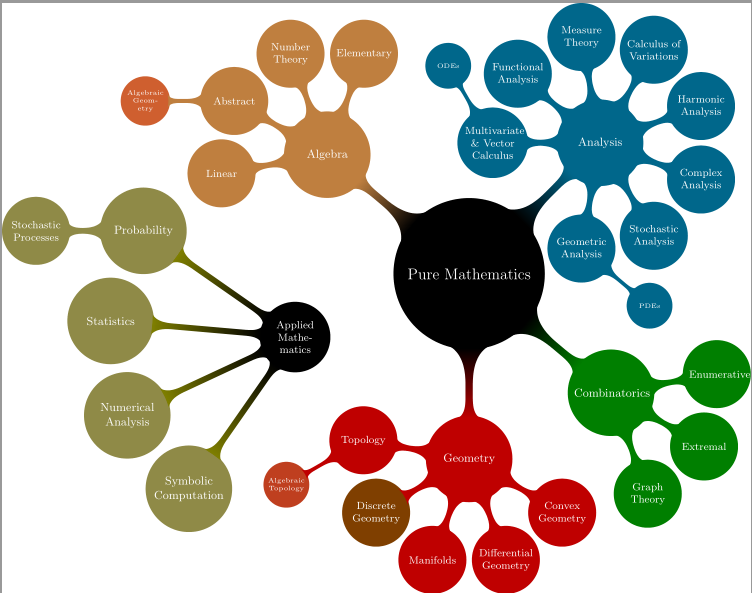
\includegraphics[width=0.8\linewidth]{mindmap.png}
	\caption{使用Tikz制作思维导图示例。}\label{fig:mindmap}
\end{figure}

\section{文档类编写}

\section{总结}

\end{document}